The first area of investigation this work seeks to tackle is how constant magnetic fields can be utilized to modify the microstructure of a bijel during formation. To achieve this goal, the extent of microstructure change that constant magnetic fields facilitate and the underlying cause for any observed microstructure change will be probed. This was accomplished through applying constant magnetic fields of strength $\Bar{B} = 0, 0.2, 0.5, 1$ in the z direction on bijels as they were phase separating. The obtained microstructure and particle order are analyzed below.

\begin{figure}[h]
    \centering
    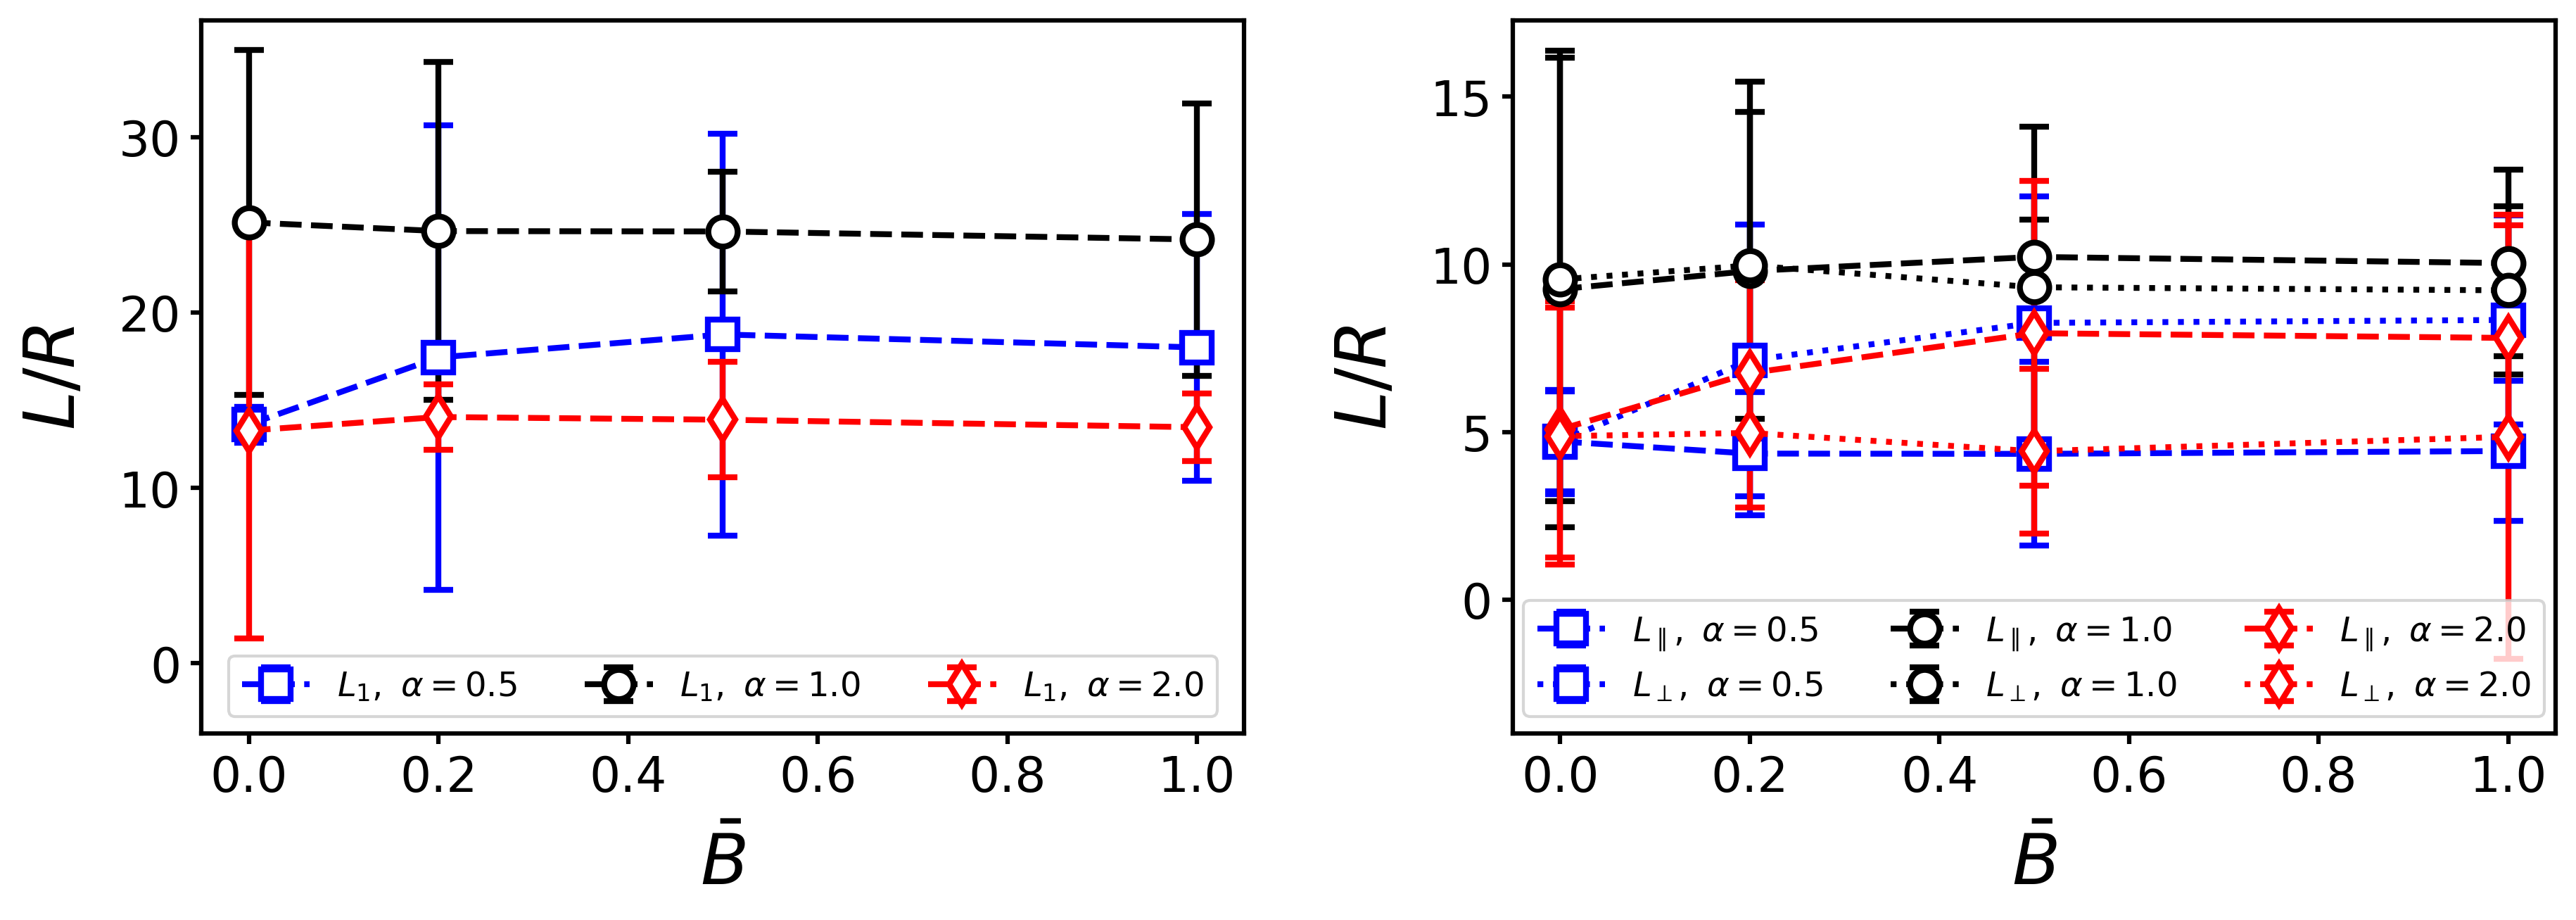
\includegraphics[scale = 0.5]{figures/results/paper1/D2a-vs-B_ss.png}
    \caption{Dimensionless average domain size ($L_1$, left) and perpendicular and parallel to the field direction domain sizes ($L_{\perp}, L_{\parallel}$, right) plotted against dimensionless magnetic field strength. Domain sizes are dimensionless by dividing with the larger radius the particle.}
    \label{fig:P1_D-vs-B-ss}
\end{figure}

Figure \ref{fig:P1_D-vs-B-ss} shows that the average domain size, $L_1$, is not significantly affected by the application of a magnetic field. Ellipsoidal particles result in smaller domain sizes compared to spherical particles, as observed by Gunther et al. This is due to their larger cross-sectional area to volume ratio, increasing interfacial coverage and causing the bijel to jam earlier. Directional domain sizes, however, show significant changes with ellipsoidal particles, varying based on particle aspect ratio. Prolate particles, with magnetic moments parallel to their long axis, show an increase in $L_{\parallel}$ by approximately $\approx 3 L/R$, while $L_{\perp}$ remains unchanged. This trend is inverted for oblate particles, with $L_{\perp}$ increasing by approximately $\approx 4 L/R$.

\begin{figure}
    \centering
    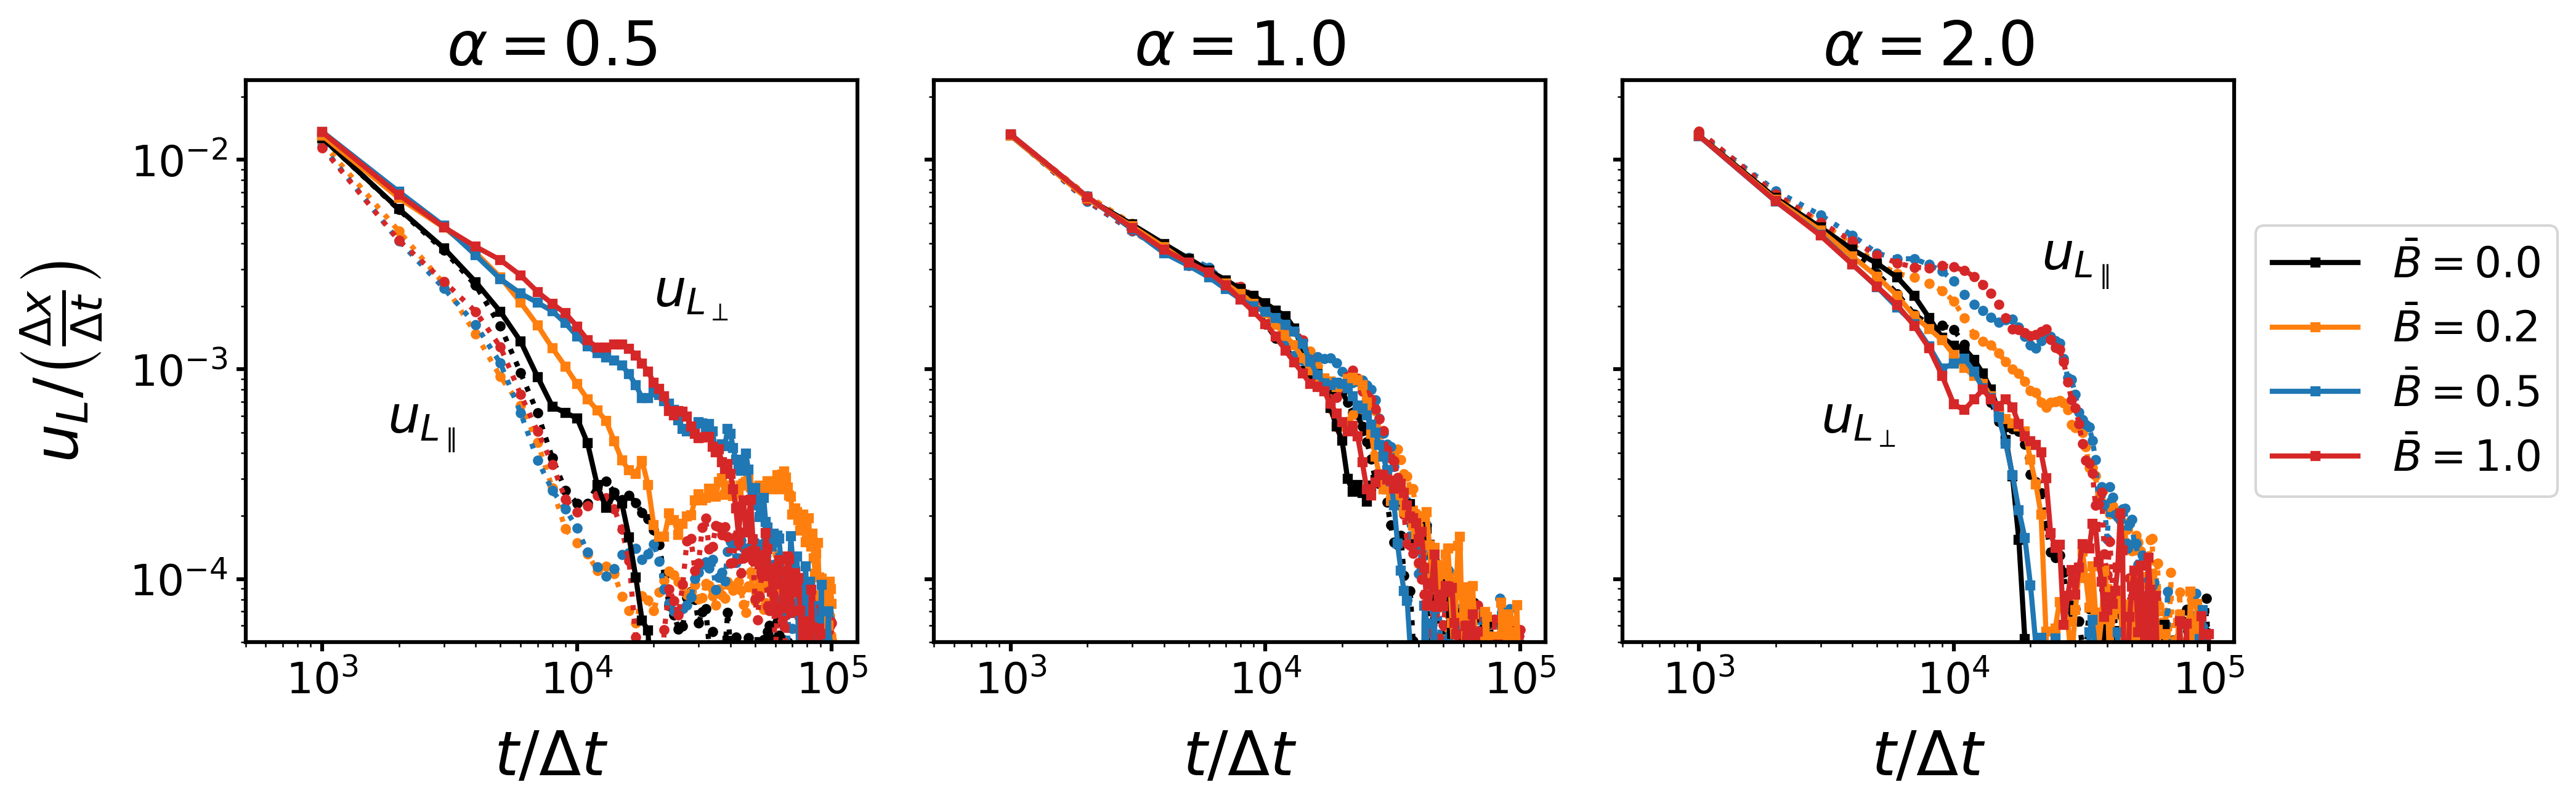
\includegraphics[scale = 0.5]{figures/results/paper1/coarsening_vel.png}
    \caption{Coarsening rates of the bijel under different field strengths over time. A coarsening rate of 0 implies a jammed system. When ellipsoidal particles are used, the jamming points in each direction change when a field is applied, especially apparent at higher field strengths.}
    \label{fig:P1_coarsen}
\end{figure}

% \begin{wrapfigure}{l}{10cm}
% \caption{Coarsening rates of the bijel under different field strengths over time. A coarsening rate of 0 implies a jammed system. When ellipsoidal particles are used, the jamming points in each direction change when a field is applied, especially apparent at higher field strengths.}
% \label{wrap-fig:P1_coarsen}
% 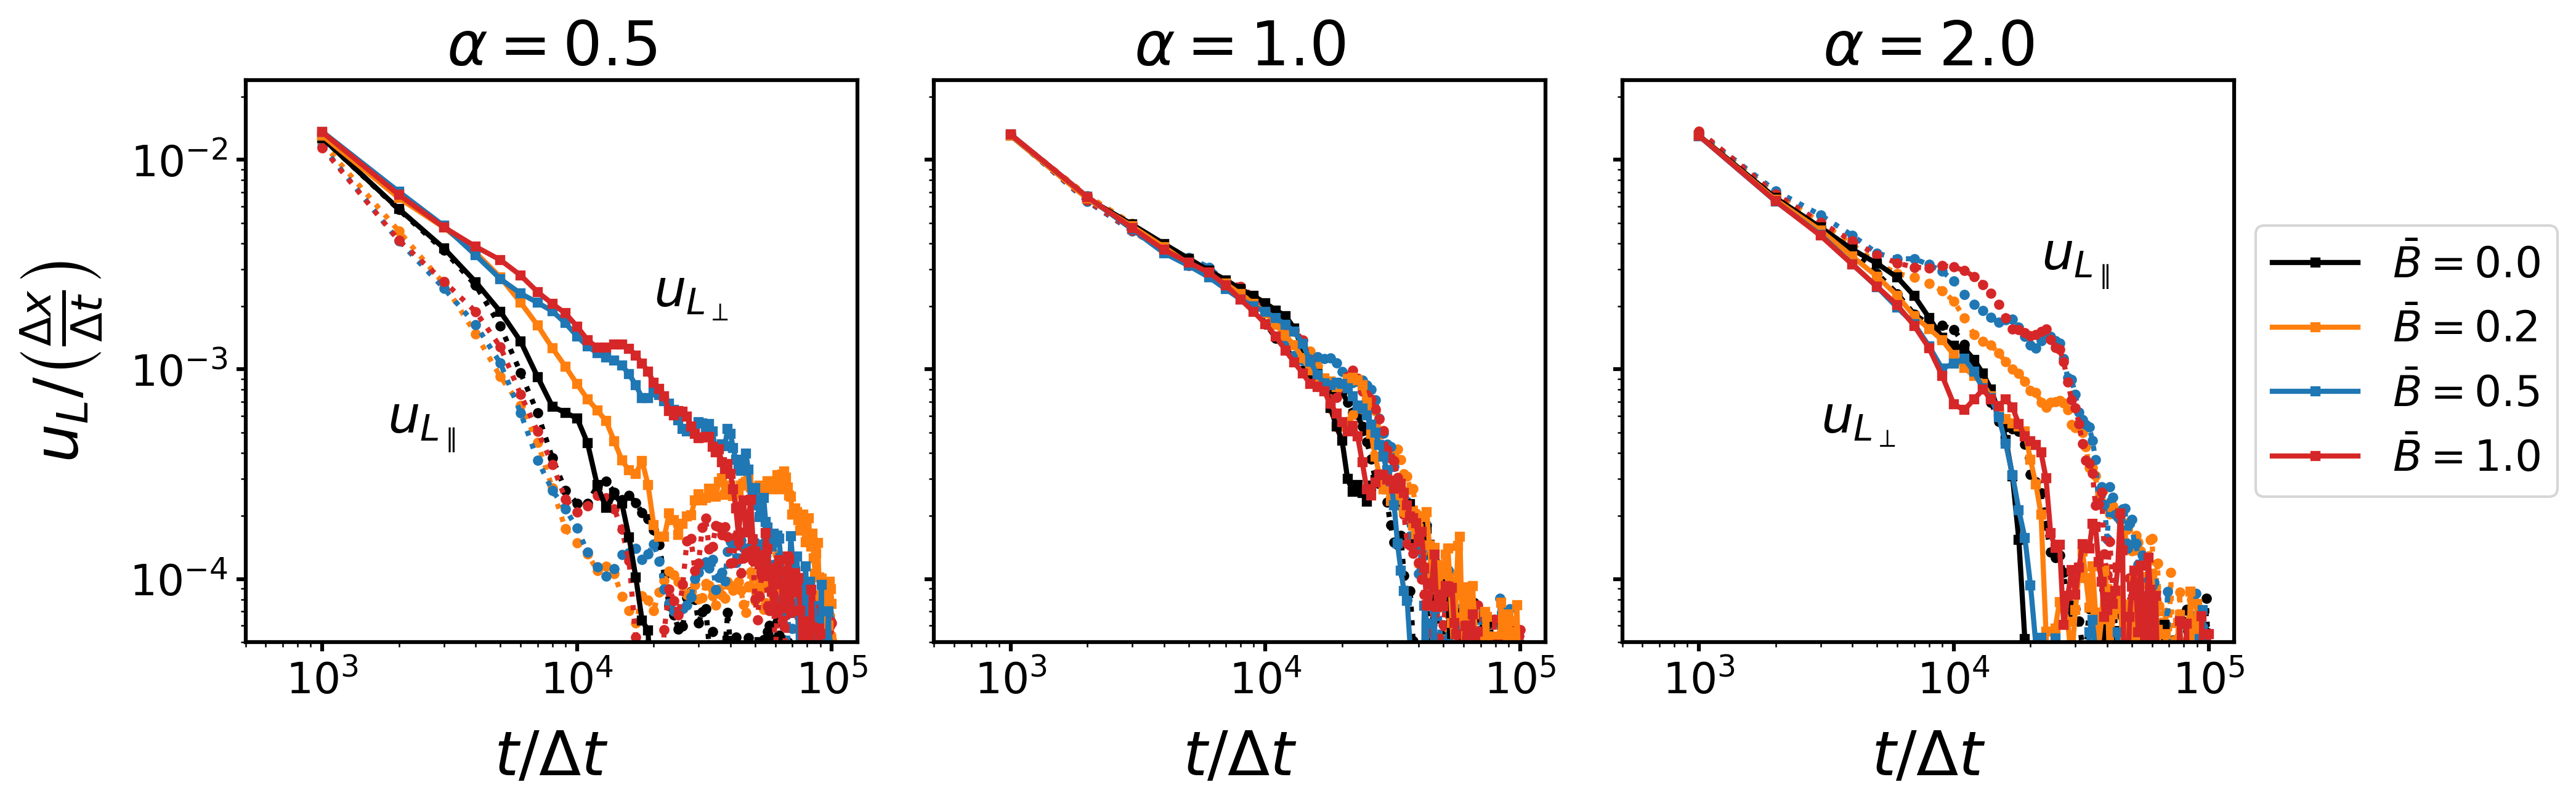
\includegraphics[width=10cm]{figures/results/paper1/coarsening_vel.png}
% \end{wrapfigure}

In this system, the microstructure is controlled through particle jamming, with any magnetic field-induced ordering observed as a change in the bijel's jamming point, defined when the coarsening rate is zero. Anisotropy in domain size indicates a divergence between directional coarsening rates. The coarsening rate, defined as the change in domain size over time, is analyzed directionally as $u_{L_{\parallel}}$ and $u_{L_{\perp}}$. Figure \ref{fig:P1_coarsen} shows that bijels stabilized with spherical particles have coarsening rates independent of field strength. However, ellipsoidal particles exhibit different coarsening rates in parallel and perpendicular directions, with the jamming point correlated to domain size. This suggests that magnetic field-driven particle ordering at the interface modifies the bijel's jamming point and microstructure.

\begin{figure}
    \centering
    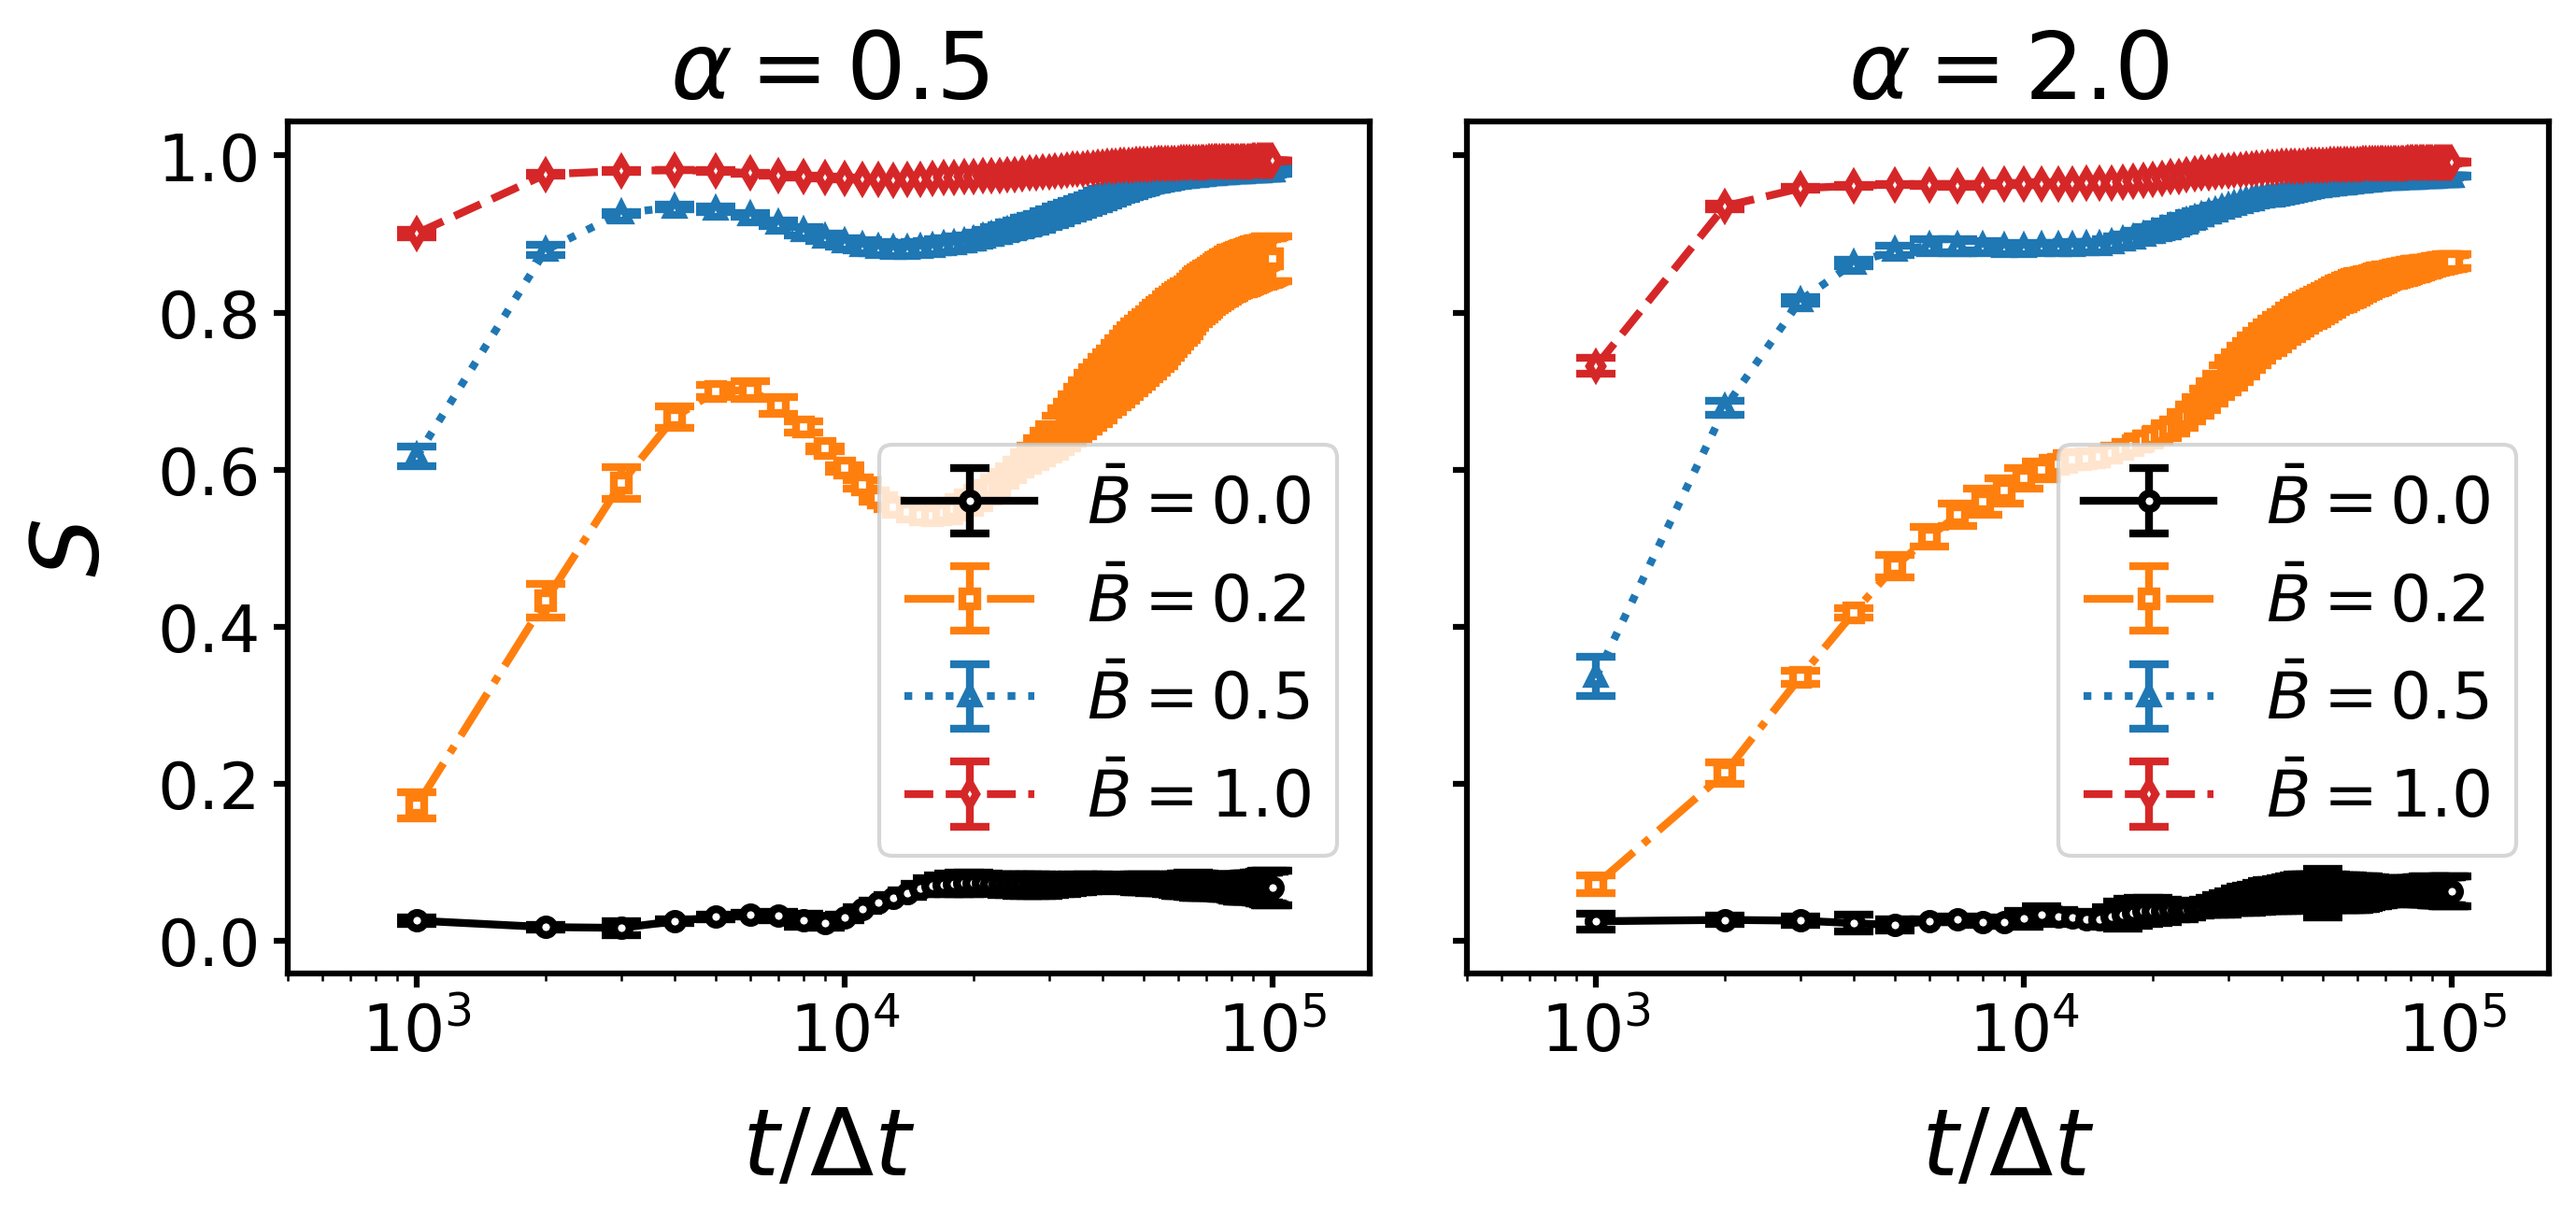
\includegraphics[scale = 0.5]{figures/results/paper1/S-vs-t.png}
    \caption{Plots of the nematic order $(S)$ of ellipsoidal particles over time. $S = 1$ indicates all particles are aligned with one another. $S \geq 0.3$ indicates an isotropic to nematic transition \cite{veerman_phase_1992}}
    \label{fig:P1_nematic}
\end{figure}

To conclusively link if particle ordering driven by the magnetic field was the cause of the change in coarsening rate, the nematic order parameter $(S)$ was used to calculate the average order of the particles over time, shown in Figure \ref{fig:P1_nematic}. As the spherical particles show no microstructure modification under an applied field, they are omitted from this plot. Figure \ref{fig:P1_nematic} shows that the nematic order of the particles increase as a function of the applied field strength. This links the ordering of the particles being caused by the applied magnetic field. The shape of the nematic ordering over time also changes as a function of the applied field, with a non-monotonic increase being seen for both ellipsoidal particles tested. Davies identified that the tilt of an ellipsoidal particle to the interface was a force balance between the interfacial and magnetic field forces. \cite{davies_interface_2014} 

\begin{figure}
    \centering
    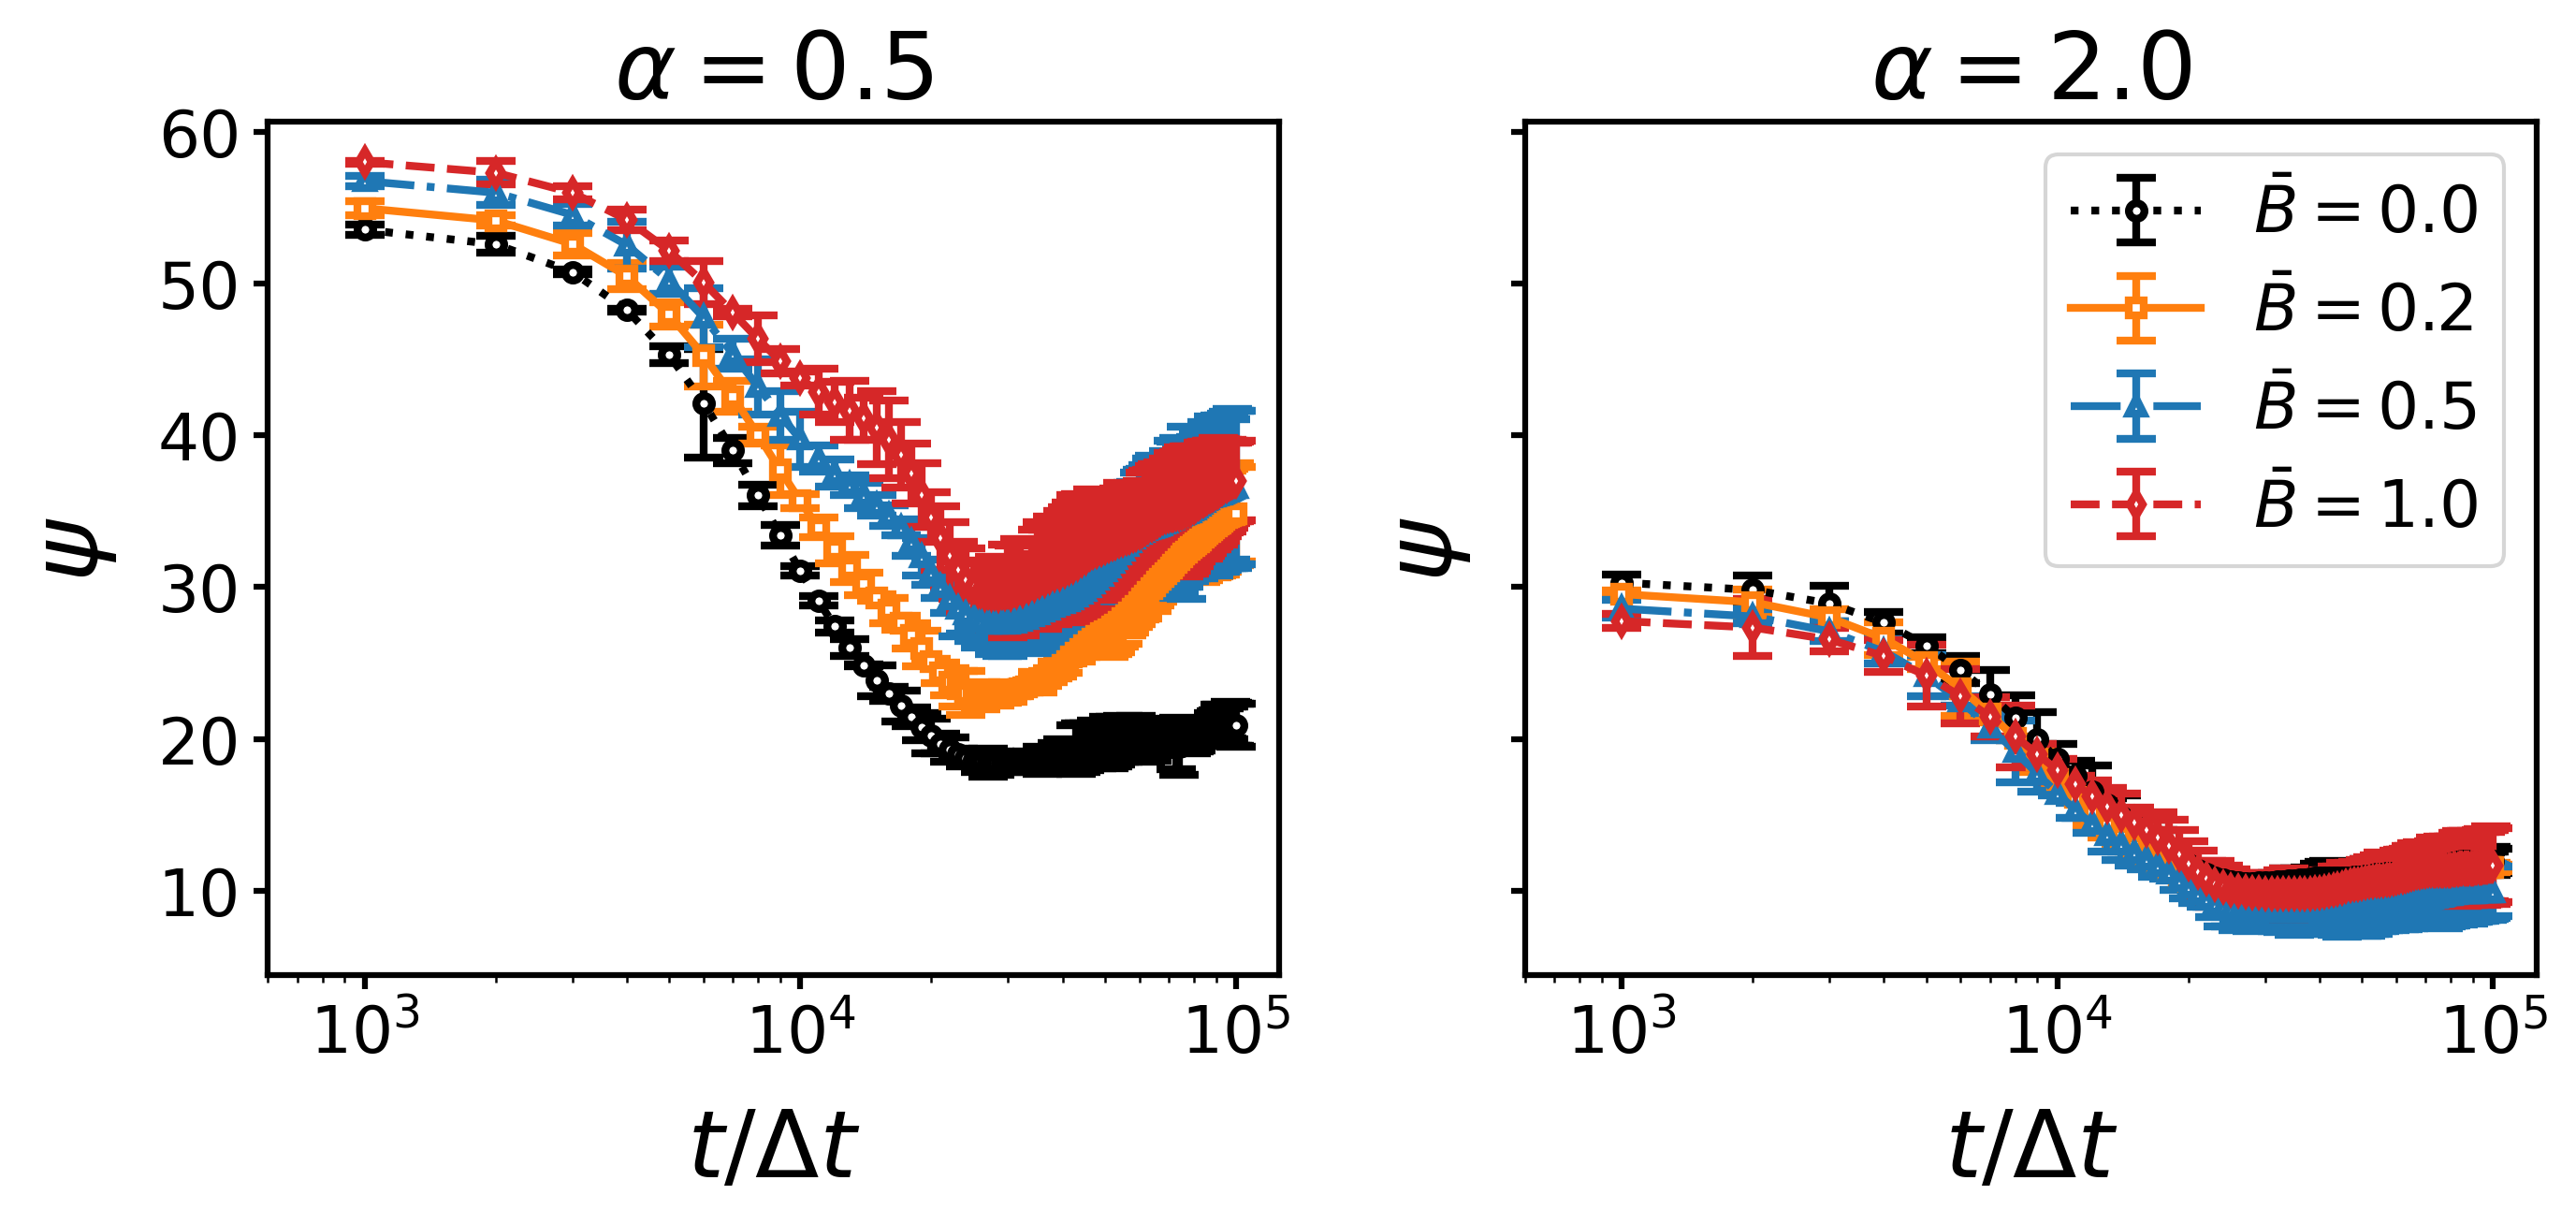
\includegraphics[scale = 0.5]{figures/results/paper1/psi-vs-t.png}
    \caption{Plots of the average angle between the particle dipole moment and interface normal $(\psi)$ over time. While there are minor changes in for the oblate particles, these are not as significant as the ordering of particles to the field.}
    \label{fig:P1_particle-angle}
\end{figure}

The non-monotonic changes seen in the nematic order parameter may be driven through a balance between steric and magnetic field forces tilting particles out of the interface to orient to the field or through the interface itself realigning particles during domain coarsening. To identify which of these mechanisms dominate in this system, the angle between the dipole moment and the interface normal $(\psi)$ is plotted. An oblate or prolate ellipsoid lying in its equilibrium orientation on the interface should have $\psi = 0 ^{\circ}$ and $\psi = 90 ^{\circ}$ respectively. From Figure \ref{fig:P1_particle-angle}, even with no field it can be seen that not all particles lie completely flat on the interface. Upon field application, the prolate particles seem to be unaffected while the oblate particles show a slight increase in the angle, demonstrating that they are tilting out of the interface more than at equilibrium. If steric and magnetic field forces dominate $\psi$ should be changing greatly with time as the interface does not remain static to the direction of the field. However, the particle orientations remained pinned to the interface, suggesting that as the particles orient to the field, the particles drag the interface with them.
